\textbf{\textit{Detector Response and Statistical Treatment}}---Neutrinos produced by SNe do not have sufficient energy to be individually resolved; however, the large number of neutrinos arriving together gives rise to a temporally localized increase in the noise rate of the detector. 
In order to simulate the signal the prreviously described models would produce, we use the \texttt{ASTERIA}~\cite{spencer_griswold_2020_3926835} software.
This program estimates the light yield from low-energy neutrinos in the IceCube Neutrino Observatory.
In order to interface with \texttt{ASTERIA}, we use the \texttt{SNEWPY} packages, which allows us to define custom supernova fluxes.

\begin{figure*}
    \centering
    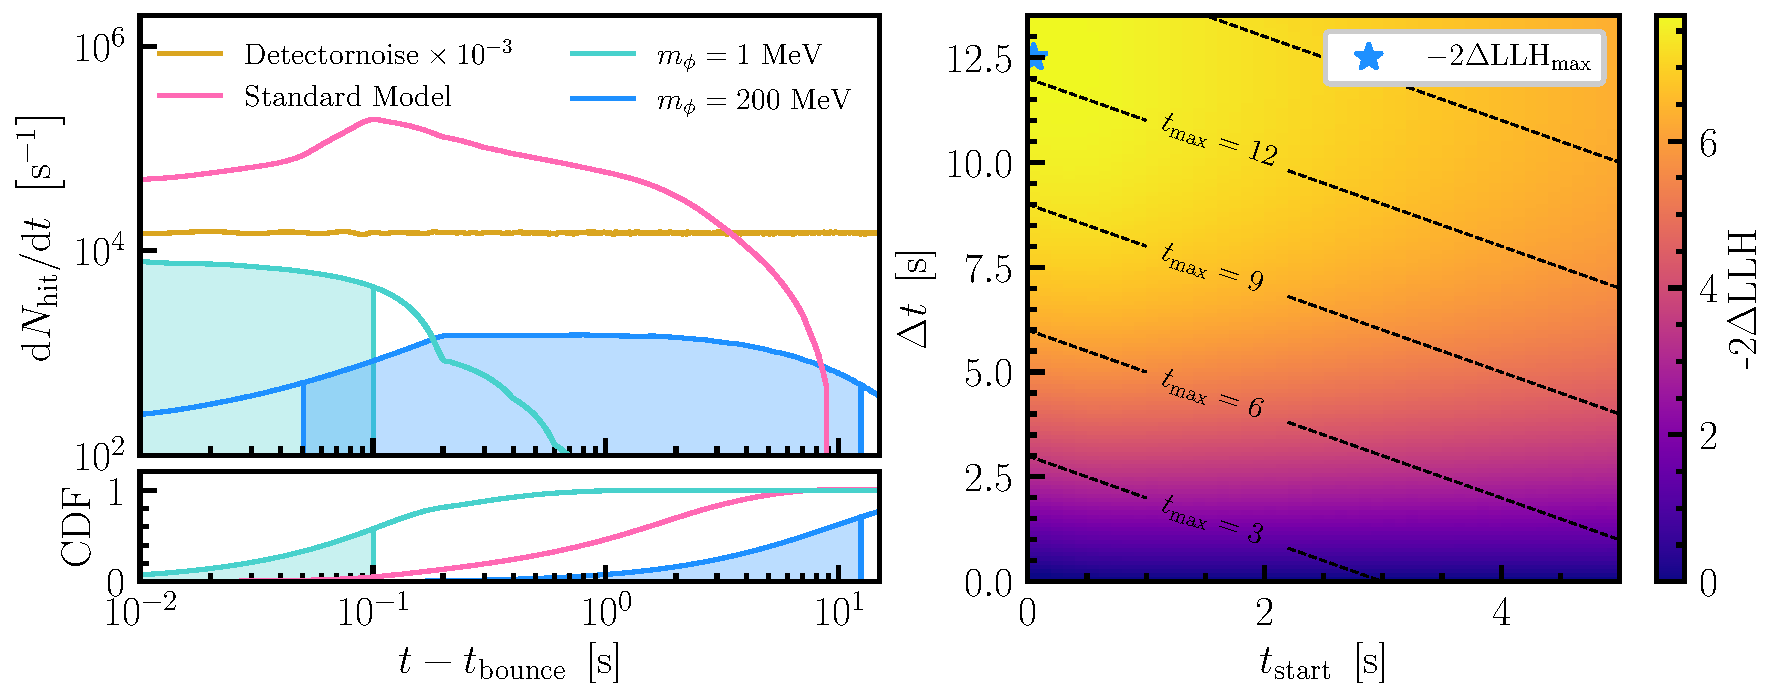
\includegraphics[width=0.95\textwidth]{figures/hits_and_likelihood.pdf}
    \caption{\textbf{\textit{Test statistic as a function of $t_{\mathrm{start}}$ and $\Delta$t.}
    }}
    \label{fig:hits_and_likelihood}
\end{figure*}